\documentclass[conference]{IEEEtran}
\IEEEoverridecommandlockouts
% The preceding line is only needed to identify funding in the first footnote. If that is unneeded, please comment it out.
\usepackage{cite}
\usepackage{amsmath,amssymb,amsfonts}
\usepackage{algorithmic}
\usepackage{graphicx}
\usepackage{textcomp}
\usepackage{xcolor}
\usepackage{url} % For better URL handling
\usepackage{xurl} % For more flexible URL breaking
\usepackage{stfloats}
\usepackage{float}
\usepackage{siunitx} % For \num command
\usepackage{booktabs} % For better table formatting
\usepackage{array}    % For column alignment
\usepackage{ragged2e} % For text justification
\usepackage{xspace}   % For proper spacing
\def\BibTeX{{\rm B\kern-.05em{\sc i\kern-.025em b}\kern-.08em
    T\kern-.1667em\lower.7ex\hbox{E}\kern-.125emX}}

\begin{document}
\title{Real Time Trade Settlement for the US Market}

\author{
    \IEEEauthorblockN{Debarshi Chakraborty\hspace{2cm}}
    \IEEEauthorblockA{
        Department of Computer Science\hspace{2cm}\\
        RKMVERI\hspace{2cm}\\
        Belur, India\hspace{2cm}\\
    }
    \and
    \IEEEauthorblockN{Chung-Sheng Li\hspace{4cm}}
    \IEEEauthorblockA{
        \textit{IEEE Fellow\hspace{4cm}}\\
        New York, USA\hspace{4cm}
    }
    \and
    \IEEEauthorblockN{\hspace{7.5cm}Rajdeep Mazumder\hspace{7.5cm}}
    \IEEEauthorblockA{
    \hspace{7.5cm}\textit{IEEE Senior Member}\hspace{7.5cm}\\
    \hspace{7.5cm}New York, USA\hspace{7.5cm}
    }
}

\maketitle


\begin{abstract}
The US market recently moved to a T+1 settlement cycle, which is quite a big step forward, but the real goal here is achieving real time settlement - basically T + 0 or instant settlement - with the ultimate goal of achieving real-time (T+0) settlement, which could significantly enhance the efficiency and stability of U.S. financial markets. This paper proposes a complete solution for instant trade settlement in the US market. Our approach involves using technologies like Distributed Ledger Technology (DLT) and Blockchain and combining them with intelligent automation using Agentic Artificial Intelligence (AI) and Large Language Models (LLMs) for their analytical power. The system being detailed here is built around a private, permissioned blockchain setup. This approach gives us immutable record keeping and atomic settlement capabilities through smart contracts. What this means is that tokenized securities and cash can be transferred instantaneously. When it comes to Agentic AI, this technology is being looked at to handle various tasks autonomously. Tasks like pre trade validation, managing real time liquidity, optimizing collateral, and dealing with post trade exceptions. These capabilities collectively aim to reduce both operational and counterparty risks. As for LLMs, these will work as intelligent interfaces for monitoring and reporting. They will handle regulatory compliance automation and improve market insights using natural language processing. This whole integrated framework being proposed should help drastically cut down counterparty risk, boost liquidity, reduce operational costs, and make things more transparent and auditable. This paper also tackles some key challenges - regulatory alignment, interoperability issues, scalability concerns, and cybersecurity aspects. This provides a realistic roadmap for where U.S. financial market infrastructure might head in the future. This work introduces a comprehensive framework that brings together permissioned distributed ledger technology, autonomous AI agents, and large language models to streamline regulatory processes. The result is a real-time (T+0) settlement system specifically designed to meet the demands of institutional trading in the U.S. financial markets.
\end{abstract}

\begin{IEEEkeywords}
Real-Time Settlement(T+0), Distributed Ledger Technology for Finance,  Agentic AI,  Smart Contract Atomic Settlement
\end{IEEEkeywords}

\section{Introduction}
Real-time trade settlement (T+0) represents the immediate and simultaneous exchange of securities and cash when a trade is executed. Unlike traditional settlement cycles where the actual transfer of ownership and funds happens one or more business days after the trade date, T+0 ensures that asset ownership and the corresponding payment are completed almost instantly. This approach eliminates the time gap that has historically exposed market participants to various types of risk.
Several factors motivate the transition toward T+0 settlement. First, it offers a substantial improvement in market efficiency. When capital and securities are freed up immediately, liquidity increases significantly, enabling market participants to redeploy their assets more quickly and make better use of their capital\cite{b1}. Second, and perhaps most importantly, real-time settlement dramatically reduces risk exposure\cite{b2}. T+0 virtually eliminates counterparty risk by ensuring atomic (all-or-nothing) delivery versus payment (DvP). It also reduces market risk since participants are no longer exposed to price fluctuations that can occur between trade execution and settlement. Finally, the push toward T+0 is driven by rapid technological advances across multiple industries, especially in distributed computing and artificial intelligence, which now provide practical ways to achieve this long-standing goal\cite{b1}. The key contribution of this work lies in its end-to-end architectural design, combining permissioned DLT, smart contracts, Agentic AI, and LLMs to create a legally compliant, scalable, and intelligent T+0 settlement system. Unlike incremental improvements, this paper proposes a modular but integrated framework capable of coexisting with or replacing existing market infrastructure.
\\\\
This continued pursuit of efficiency has found a powerful enabler in the rise of Distributed Ledger Technology (DLT). DLT, with its ability to create shared, immutable, and cryptographically secured records, provides the foundational infrastructure necessary to underpin a truly real-time settlement system. According to Goldman Sachs (2016), DLT could reduce transaction costs of insurance underwritings by \$2–4 billion in the USA alone and the costs related to securities clearing and settlement would decrease by \$11–12 billion. An analysis of Banco Santander, Oliver Wyman, and Anthemis Group (2015) suggests that DLT could reduce banks’ infrastructure costs attributable to cross-border payments and trading of securities by \$15–20 billion. The World Economic Forum (2015) even estimates that by 2027, up to 10\% of the value of the global GDP will be stored on blockchains\cite{b3}.

\section{Background and Motivation}
The evolution of trade settlement in the U.S. reflects a persistent drive toward improved efficiency, lower risk, and smarter use of technology. What started as a mostly manual process involving lots of paperwork has gradually become a highly automated system, with settlement times getting shorter and shorter between when a trade happens and when it is actually finalized.
\begin{figure}[htbp]
    \centering
    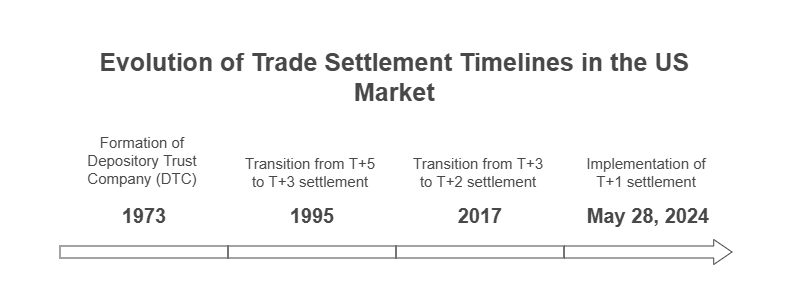
\includegraphics[width=0.4\textwidth]{1.png}
    \caption{Reduction in settlement times across decades}
    \label{fig:settlement_timeline}
\end{figure}
\subsection{Traditional Clearing and Settlement Processes}
In the traditional framework, several specialized entities play vital roles in bringing a trade from execution to final settlement:

\begin{itemize}
    \item \textbf{Brokers}: Execute client orders and facilitate trade matching
    \item \textbf{Custodians}: Safeguard assets and handle administrative services
    \item \textbf{CCPs}: Act as central intermediaries to mitigate counterparty risk
    \item \textbf{CSDs}: Maintain electronic securities records and enable book-entry transfers
\end{itemize}
The traditional settlement process can be broadly divided into three main phases:
\begin{itemize}
    \item \textbf{Trade Execution}
     \item \textbf{Clearing}
      \item \textbf{Settlement}
\end{itemize}
\begin{figure}[H]
    \centering
    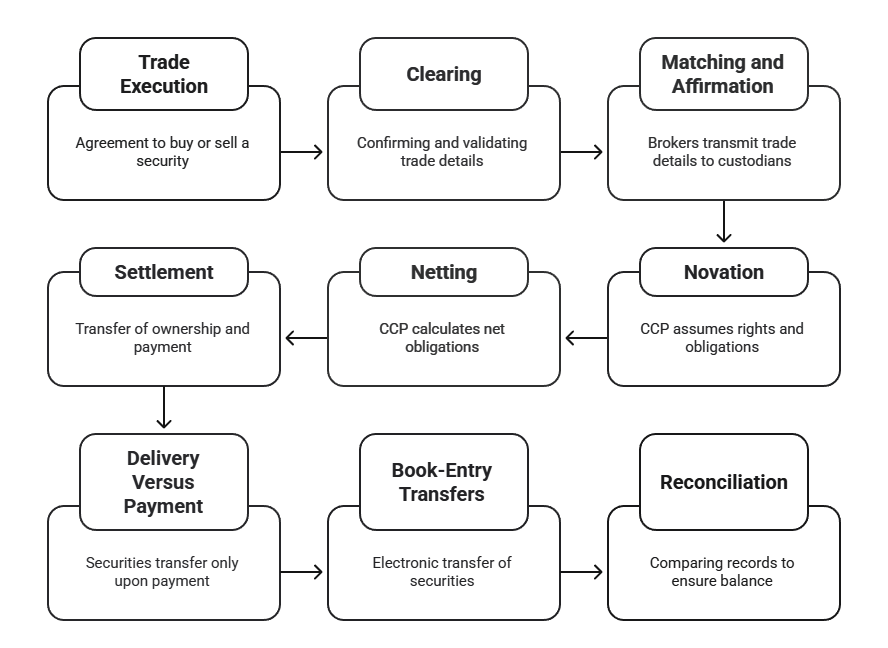
\includegraphics[width=0.5\textwidth]{2.png}
    \caption{Trade Settlement Process}
    \label{fig:settlement_timeline}
\end{figure}
\section{System Architecture and Design}
The shift toward real-time (T+0) settlement demands more than incremental upgrades — it requires reimagining the post-trade infrastructure from the ground up. To that end, the proposed system presents a distributed architecture that tightly integrates tokenized financial instruments, smart contract automation, agentic AI-driven validation, and LLM-assisted compliance. The system is designed for deployment on a private, permissioned blockchain network, with deterministic consensus and compliance-layer observability at its core.

In what follows, we outline each component of this architecture, drawing from real-world DLT standards (e.g., ERC-1400 for security tokens, ERC-20 for cash equivalents), and layering them with intelligent execution logic via smart contracts and autonomous agents.
\subsection{Tokenization of Assets}
The foundational step involves the tokenization of both securities and cash. This means that each share of stock, bond, or unit of currency is represented as a unique, programmable digital token. The proposed system relies on the \textbf{ERC-1400} standard (or similar domain-specific variants) for tokenized securities, allowing support for compliance checks, partitions, and transfer restrictions. The cash leg follows the more straightforward \textbf{ERC-20} representation, backed by pre-funded digital deposit accounts or stablecoin equivalents.

All tokens reside on a permissioned Ethereum-compatible ledger, such as \textbf{Hyperledger Besu}, enabling enterprise-grade privacy and access control while preserving the benefits of distributed consensus and auditability.
\subsection{Trade Execution and Smart Contract Initiation}
Once two participants reach an execution agreement, a digitally signed transaction is generated and submitted to the settlement layer. This triggers a pre-deployed smart contract, parameterized with the trade specifics.

Smart contracts are authored in \textbf{Solidity}, rigorously tested via \textbf{Hardhat} and integrated with access control modules to ensure only authorized contract factories can deploy settlement logic. Each contract encodes atomicity conditions, timeouts, and compliance gating functions.
\subsection{Rationale for Agentic AI} 
Agentic AI offers a superior alternative to traditional automation by autonomously resolving compliance checks, liquidity mismatches, or collateral issues in real time. Unlike static rule-based systems or black-box ML models, Agentic AI is context-aware, explainable, and capable of triggering smart contract workflows or escalating to human review. This autonomy is crucial for achieving seamless T+0 operations under varying market conditions
\subsection{Immediate Trade Validation (Agentic AI \& Consensus Mechanisms)}
Upon receiving a settlement instruction, the participating firms’ Agentic AI modules begin validation — concurrently and without manual intervention. Each module performs:
\begin{itemize}
    \item \textbf{Inventory checks} using read-only queries to the respective wallet balances.
    \item \textbf{Real-time credit} exposure analysis, using internal risk models and historical volatility data.
    \item \textbf{Compliance rule enforcement}, using embedded rule parsers and policy dictionaries.
\end{itemize}

If any discrepancies or potential issues are found, the Agentic AI would either:
\begin{itemize}
    \item Proactively resolve: Initiate an automated liquidity solution like a pre-approved, instant intra-firm transfer of tokens or a tokenized collateral loan via another smart contract.
    \item Flag for human review: If a complex issue arises, an LLM could generate a concise summary of the problem and potential solutions for human intervention.
\end{itemize}

Concurrently, the DLT's consensus mechanism rapidly validates the proposed transaction across the distributed network of participants. This ensures that all nodes agree on the validity and order of the transaction.

\subsection{Atomic Settlement via Smart Contract}
Following consensus, the smart contract enters its atomic execution phase. Here, the \textbf{transferFrom()} function is invoked on both the ERC-1400 (security) and ERC-20 (cash) contracts. The contract ensures simultaneity using a commit-reveal or hashed secret scheme, preventing partial execution.
If either leg fails—for example, due to a token shortfall or unexpected permission error—the transaction auto-rolls back, ensuring no assets move unilaterally. The system specifically avoids optimistic rollups or probabilistic finality mechanisms here, as financial settlement must be deterministic and legally binding.

Every successful transaction emits an event log that is indexed on-chain and optionally broadcast via \textbf{Kafka queues or webhooks} to the participants' back-office systems.

\subsection{Post-Settlement Automation and Reporting (Agentic AI \& LLMs)}
Immediately upon finalization, the Agentic AI systems trigger internal subledger updates. The system event-driven architecture for post-settlement bookkeeping — each emitted event invokes an internal process (using something like \textbf{Apache Airflow or AWS Step Functions}) to reconcile trade status, update exposure dashboards, and notify treasury desks.
Simultaneously, LLMs generate:
\begin{itemize}
    \item Regulatory filings.
    \item Real-time audit logs.
    \item Explanatory summaries for compliance teams.
\end{itemize}
These models operate on \textbf{retrieval-augmented generation (RAG)} pipelines, querying from vectorized corpora of regulatory texts indexed using \textbf{FAISS or Qdrant}. The system also performs anomaly detection — flagging, for instance, unusually fast token turnover or suspicious cross-trading patterns — using a combination of \textbf{EWMA-based thresholds, autoencoders, and graph-based transaction tracing}.
\begin{figure}[H]
    \centering
    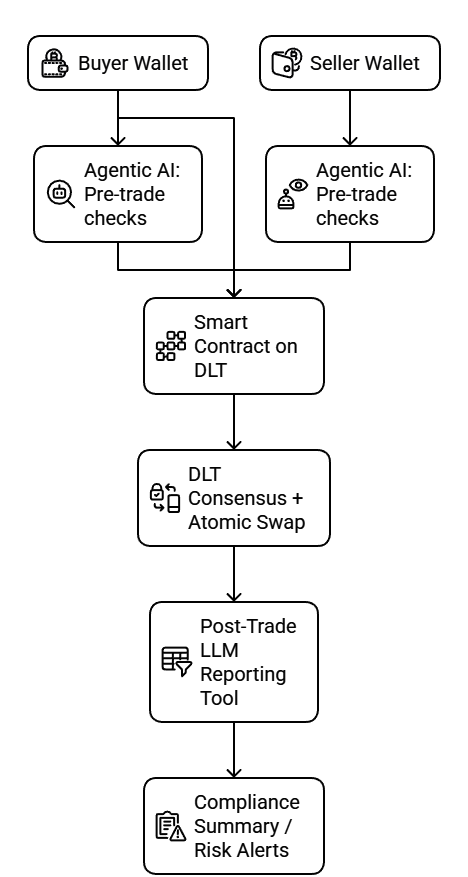
\includegraphics[width=0.3\textwidth]{3.png}
    \caption{T+0 settlement using Blockchain, DLT, AI Agents and LLMs}
    \label{fig:settlement_timeline}
\end{figure}
\section{Consensus Choice and Finality Requirements}
A key requirement for regulated financial settlement systems is \textbf{deterministic finality}-that is, the absolute guarantee that once a transaction is confirmed, it cannot be reversed. This is especially critical for Delivery-versus-Payment (DvP) in securities transactions, where atomic settlement is legally and operationally essential\cite{b4}.

\subsection{IBFT-2 Consensus Protocol}
For the architecture, the system adopts the Istanbul Byzantine Fault Tolerance version 2 (IBFT-2) consensus protocol, as implemented in the Hyperledger Besu client. IBFT-2 is a permissioned consensus mechanism that tolerates up to $\lfloor(n-1)/3\rfloor$ faulty nodes and guarantees finality in a bounded number of rounds. According to empirical evaluations by the Besu community and Hyperledger documentation, transaction finality is typically achieved within 1-2 seconds, depending on block size and node network latency.

\subsection{Comparison with Alternative Mechanisms}
IBFT-2 was selected over probabilistic mechanisms like Proof-of-Stake (PoS) or Proof-of-Work (PoW) because the latter cannot guarantee absolute finality within a finite timeframe. For example:
\begin{itemize}
    \item Ethereum's PoS-based consensus introduces probabilistic finality with chain reorg risk
    \item This is unsuitable for financial markets requiring legally binding settlement with finality guarantees
\end{itemize}

In contrast, IBFT-2 enables:
\begin{itemize}
    \item Regulators and market participants to rely on each block's confirmation as legally final
    \item Significant reduction in systemic and operational risk
\end{itemize}

\subsection{Performance Characteristics}
Additionally, IBFT-2 supports:
\begin{itemize}
    \item Low-latency block production ($<2$ seconds)
    \item Crucial for real-time (T+0) settlement scenarios
    \item Scalability for high-volume U.S. equity markets
\end{itemize}

\section{Quantitative Risk Analysis}

To quantify the risk reduction from transitioning from T+1 to T+0 settlement, this paper implements a Monte Carlo simulation using historical settlement failure rates and trade characteristics observed in U.S. markets. The simulation compares expected counterparty exposure measured in \textbf{dollar-hours} under both settlement regimes.

\subsection{Model Assumptions}

\begin{itemize}
    \item \textbf{Average Trade Value:} Each simulated trade assumes an average notional value of \$1,000,000, reflecting institutional block trade sizes commonly observed in U.S. equity markets, and aligning with SIFMA benchmarks for institutional order flows.
    
    \item \textbf{Trade Value Distribution:} Trade sizes are sampled from a log-normal distribution to realistically capture the positive skew and heavy-tailed nature of trade volumes—features well-documented in empirical market microstructure literature.
    
    \item \textbf{Failure Modeling:} Settlement failures are modeled using a Bernoulli process with a historical fail rate of $p = 0.0019$ (0.19\%), derived from industry-reported averages and regulatory filings. This reflects a conservative but realistic failure likelihood under T+1 conditions.
    
    \item \textbf{Exposure Definition:} Counterparty exposure is calculated only in cases of settlement failure and is assumed to scale proportionally with both the trade value and the time-to-finality. The exposure window is reduced from 24 hours (T+1) to 2 hours (T+0), reflecting the latency guarantees of deterministic consensus protocols like IBFT-2.
\end{itemize}


\subsection{Simulation Methodology}

For each simulated trade $i$:

\begin{align}
    V_i &\sim \text{LogNormal}(\mu, \sigma^2) \quad \text{(Trade Value)} \\
    F_i &\sim \text{Bernoulli}(p) \quad \text{(Settlement Failure Event)} \\
    E_i^{\text{T+1}} &= V_i \cdot F_i \cdot T_{1}, \quad T_{1} = 24 \text{ hours} \\
    E_i^{\text{T+0}} &= V_i \cdot F_i \cdot T_{0}, \quad T_{0} = 2 \text{ hours} \\
    R_i &= E_i^{\text{T+1}} - E_i^{\text{T+0}} \quad \text{(Risk Reduction)}
\end{align}

We simulate $N = 10{,}000$ trades, where each trade value is drawn from a log-normal distribution with parameters $\mu = \log(10^6)$ and $\sigma = 0.5$. The expected daily exposure and risk reduction are given by:


\begin{align}
    \mathbb{E}[E^{\text{T+1}}] &= \frac{1}{N} \sum_{i=1}^{N} E_i^{\text{T+1}} \\
    \mathbb{E}[E^{\text{T+0}}] &= \frac{1}{N} \sum_{i=1}^{N} E_i^{\text{T+0}} \\
    \mathbb{E}[R] &= \frac{1}{N} \sum_{i=1}^{N} R_i
\end{align}

Annualized exposure is projected by multiplying daily metrics by $D = 252$ trading days:

\begin{equation}
    \text{Annual Exposure} = \mathbb{E}[E] \cdot D
\end{equation}

The percentage reduction in exposure under T+0 is:

\begin{equation}
    \text{Risk Reduction (\%)} = \left( \frac{\mathbb{E}[R]}{\mathbb{E}[E^{\text{T+1}}]} \right) \cdot 100
\end{equation}

\subsection{Simulation Results}

Based on the simulation:

\begin{itemize}
    \item \textbf{Effective Fail Rate:} 0.20\%
    \item \textbf{Average Daily Exposure:} 
    \begin{itemize}
        \item T+1: \$57,354 dollar-hours
        \item T+0: \$4,779 dollar-hours
    \end{itemize}
    \item \textbf{Annual Risk Reduction:} 
    \begin{itemize}
        \item \$13.2 million-dollar-hours (91.7\%)
    \end{itemize}
    \item \textbf{95th Percentile Stress Scenario:} 
    \begin{itemize}
        \item T+1 Exposure: \$51.2 million-dollar-hours
        \item T+0 Exposure: \$4.3 million-dollar-hours
    \end{itemize}
\end{itemize}
\begin{figure}[H]
    \centering
    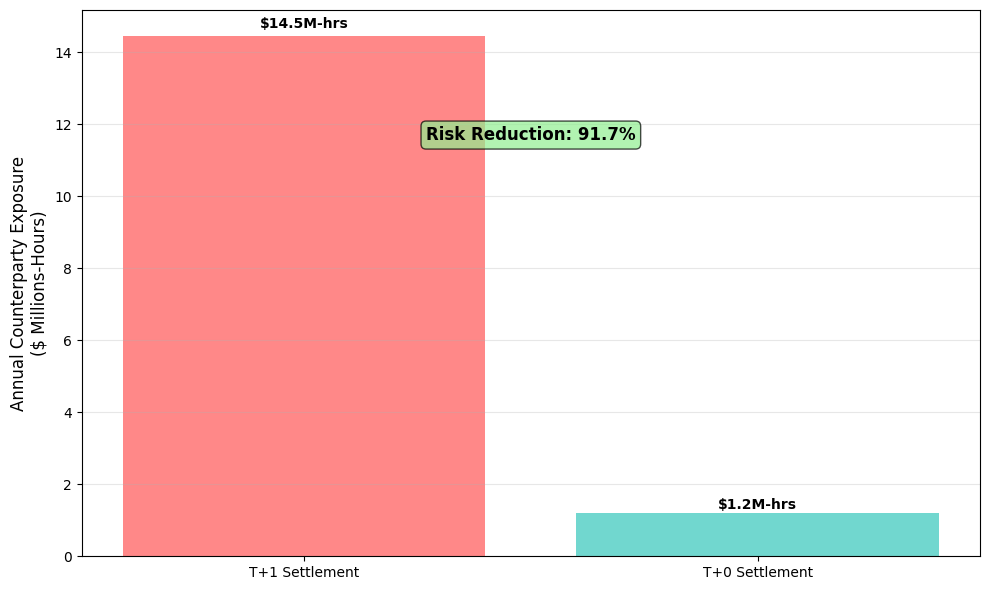
\includegraphics[width=0.5\textwidth]{output.png}
    \caption{Settlement Risk Comparison: T+1 vs T+0}
    \label{fig:settlement_timeline}
\end{figure}

\subsection{Interpretation}

The Monte Carlo simulation highlights the systemic risk implications of T+1 settlement by quantifying unsecured counterparty exposure. Under T+0, the exposure window shortens from 24 to 2 hours, resulting in a dramatic risk reduction of over 91\% annually. This reduction strengthens the argument for transitioning toward real-time or same-day settlement, particularly when weighed against cost, technological, and operational feasibility.

\section{Comparative Case Studies and Feasability Evidence}
Having established the technical framework for real-time settlement, this paper examines its practical implementation through representative case studies that demonstrate the system's viability across different market contexts.
\subsection{JPMorgan's Kinexys}
JPMorgan Kinexys (formerly Onyx) is a suite of blockchain-based solutions designed to revolutionize institutional finance. It operates by digitizing money and assets on a secure, permissioned blockchain, enabling faster, cheaper, and more transparent transactions\cite{b5} \cite{b6}.
\subsubsection{Kinexys Digital Payments}
\begin{itemize}
    \item \textbf{Tokenization \& Funding}: Clients fund ``Blockchain Deposit Accounts'' (BDAs) by transferring fiat currency from traditional accounts. This tokenizes the currency on the blockchain, creating digital representations.
    
    \item \textbf{Instant, Atomic Settlement}: Payments between BDAs or to traditional accounts occur instantly and atomically. This means transactions are either fully completed or entirely reversed, eliminating settlement risk and delays.
    
    \item \textbf{Programmable Payments}: Clients can automate complex payment flows using ``if-this-then-that'' logic, allowing for dynamic funding, event-based payouts, and real-time treasury management.
    
    \item \textbf{On-Chain FX}: Integration with FX services enables near real-time foreign exchange and settlement directly on the blockchain, reducing FX risk.
\end{itemize}
\subsubsection{Kinexys Digital Assets}
\begin{itemize}
    \item \textbf{Asset Tokenization}: Traditional financial assets are represented as digital tokens on the blockchain.
    
    \item \textbf{Enhanced Liquidity \& Mobility}: Tokenized assets can be moved, traded, and used as collateral instantly, improving liquidity and efficiency.
    
    \item \textbf{Programmable Assets}: Smart contracts embed rules into these digital assets, enabling automated actions like instant settlement .
\end{itemize}
\subsection{Fnality International}
The Sterling Fnality Payment System (£FnPS) is the first fully regulated, distributed ledger technology-based payment system in the world\cite{b7}. This marks a fundamentally different approach to financial transactions , the £FnPS is not just a new platform,but a fundamentally different approach to financial transactions, leveraging the strength of blockchain technology in a regulated environment\cite{b8}.


\subsubsection{Tokenization \& Funding: Central Bank Money on-chain}

\begin{itemize}
\item \textbf{Mechanism}: Instead of commercial bank money, Fnality's system is backed 1:1 by funds held at a central bank. This means participating financial institutions fund their balances within the Fnality Payment System by transferring traditional central bank money into an omnibus account at the respective central bank .

\item \textbf{Digital Representation}: This creates digital representations of central bank money on the blockchain, allowing for the direct use of central bank liquidity in DLT-based transactions.
\end{itemize}

\subsubsection{Real-Time, Atomic Settlement}

\begin{itemize}
\item \textbf{Atomic Settlement}: Fnality enables atomic settlement for financial transactions. This means that the exchange of digital cash for digital assets happens simultaneously, eliminating settlement risk and the need for intermediaries to guarantee each leg of the transaction.

\item \textbf{Earmarking Feature}: To further enhance atomicity, Fnality has introduced an "earmarking" feature. This allows an amount of tokenized currency to be reserved or "earmarked" for a particular transaction at a specified time, ensuring funds are available when the atomic settlement occurs. This is particularly important for securities transactions that might fail due to insufficient funds, potentially incurring penalties.
\end{itemize}
\subsection{DTCC's Project Ion}
DTCC's Project Ion is a significant initiative by the Depository Trust \& Clearing Corporation, the central post-trade market infrastructure for the U.S. securities industry. Unlike JPMorgan's Kinexys or Fnality which focus on tokenized cash or assets, Project Ion is designed as an alternative settlement platform leveraging Distributed Ledger Technology (DLT) for equity securities, operating in parallel to DTCC's existing "classic" settlement systems.
\subsubsection{Parallel Ledger, Bilateral Transactions and Underlying Technology}
\begin{itemize}
    \item  \textbf{Parallel Book}:Project Ion functions as a parallel book and infrastructure to the existing DTCC classic settlement system. This means that while trades are processed and settled on the traditional system (which remains the authoritative record), a copy or representation of these transactions is also recorded on the DLT platform\cite{b9}\cite{b10}.
    \item \textbf{Focus on Bilateral Deliveries}:Initially, Project Ion has been used for processing a segment of bilateral equity transactions between DTC participants. 
   This allows DTCC to test the DLT's capabilities in a real-world environment without disrupting the core, critical settlement infrastructure. For instance, it has processed over 100,000 bilateral equity transactions per day, and up to 160,000 on peak days, in this parallel environment\cite{b9}.
    \item \textbf{Underlying Technology}:Project Ion was developed in partnership with R3, leveraging their Corda DLT software\cite{b9} \cite{b11}. Corda is a private, permissioned DLT platform, well-suited for regulated financial environments due to its privacy features and focus on bilateral agreements.
\end{itemize}


\section{Legal and Regulatory Considerations}
The implementation of real-time settlement necessitates strict adherence to evolving financial regulations, requiring a framework that addresses three critical dimensions: compliance, risk mitigation, and auditability.
\subsection{Legal Considerations}

\begin{itemize}
    \item \textbf{Adapting to Existing Laws}:
    \begin{itemize}
        \item The current legal framework was built around traditional delayed settlement cycles. 
        \item Transitioning to a T+0 environment will likely require not only a re-interpretation of existing laws but also possible updates to legislation to support real-time processes.
    \end{itemize}
    
    \item \textbf{Evolving Legal Definitions}:
    \begin{itemize}
        \item Key financial terms such as ``account,'' ``transfer order,'' and ``finality'' have been shaped by legacy systems. 
        \item With DLT-based settlement, these terms may need to be reconsidered or redefined to reflect the nature of blockchain-based transactions.
    \end{itemize}
    
    \item \textbf{Clarifying Liability and Dispute Mechanisms}:
    \begin{itemize}
        \item Real-time systems introduce new types of risk. It is important to clearly define who is responsible in the event of technical failures, operational errors, or legal disputes.
    \end{itemize}
\end{itemize}

\subsection{Regulatory Considerations}

\begin{itemize}
    \item \textbf{Redefining ``Securities'' and ``Money''}:
    \begin{itemize}
        \item Regulatory definitions of financial instruments and currency have been shaped around physical or centrally recorded forms. 
        \item Tokenized assets and digital representations of money on a blockchain may not align neatly with these definitions, creating ambiguity about how existing regulations apply.
    \end{itemize}
    
    \item \textbf{Determining Legal Finality}:
    \begin{itemize}
        \item In traditional finance, legal finality is often achieved through central depositories or clearing mechanisms. 
        \item With DLT, the concept of when a transaction becomes legally binding and irreversible needs to be clearly defined to avoid legal uncertainty.
    \end{itemize}
    
    \item \textbf{Ownership and Custody in Digital Contexts}:
    \begin{itemize}
        \item While distributed ledgers can track asset ownership, the legal recognition of such records-especially when tied to real-world assets must be formally established. 
        \item Challenges such as proving possession of digital assets and handling scenarios involving lost or stolen private keys also require clear legal treatment.
    \end{itemize}
\end{itemize}

\begin{table*}[t]
\centering
\caption{Regulatory Compliance Framework for T+0 Settlement}
\label{tab:regulatory}
\begin{tabular}{@{}>{\RaggedRight}p{3cm}>{\RaggedRight}p{3.5cm}>{\RaggedRight}p{7cm}>{\RaggedRight}p{1.5cm}@{}}
\toprule
\textbf{Regulation/Guideline} & \textbf{Requirement} & \textbf{Proposed Control/Design Response}  \\
\midrule
SEC Rule 17Ad-22(e)(12) (Clearing Agencies) & Ensure timely and accurate settlement & Deterministic DLT finality $\leq$ 2 seconds via IBFT-2 consensus; atomic DvP via smart contracts  \\

SEC Rule 17Ad-22(e)(3) & Manage credit and liquidity risks & Real-time risk scoring and exposure control using AI-based predictive analytics; no overnight risk in T+0  \\

Federal Reserve: Payment System Risk Policy & Support real-time settlement with finality & Use of permissioned DLT ensuring pre-funded tokenized cash leg, settlement finality built into the consensus mechanism \\


Securities Exchange Act Rule 15c3-3 & Safeguard customer assets & Token custody logic enforces segregated ownership with transparent auditability on-chain  \\

FINRA Regulatory Notice 20-23 (Artificial Intelligence) & Ensure model explainability and compliance & All AI trade recommendations and settlement decisions logged and explainable; human-in-the-loop for override  \\
\bottomrule
\end{tabular}
\end{table*}
\section{Cross Jurisdiction Snapshot}
While the United States is actively modernizing its post-trade infrastructure through initiatives like DTCC’s Project Ion and private efforts such as J.P. Morgan’s Kinexys, other global jurisdictions are exploring complementary regulatory pathways. The European Union launched its DLT Pilot Regime under the Markets in Financial Instruments Regulation (MiFIR), enabling regulated trading and settlement of tokenized financial instruments on permissioned ledgers. Notably, it allows central securities depositories (CSDs) to operate DLT-based settlement systems under a regulatory sandbox until 2026, offering a risk-controlled environment for testing real-time settlement models\cite{b12}. \\\\In Singapore, the Monetary Authority of Singapore (MAS) leads Project Guardian, a public-private initiative that explores asset tokenization and DeFi protocols within a regulatory framework. MAS's focus lies in tokenizing government securities, foreign exchange, and cross-border settlements with live trials involving institutions like DBS and J.P. Morgan\cite{b13}.\\\\ Compared to the U.S. approach—which is currently led by industry consortia under existing regulatory frameworks—the EU and Singapore models are more sandbox-driven and regulator-led, enabling rapid experimentation under controlled risk. This divergence highlights the strategic trade-offs between regulated innovation versus market-led transformation, providing a broader lens for evaluating policy alignment in future DLT-based financial markets.

A key advantage of the proposed system lies in its flexibility to operate under different regulatory regimes. Its modular structure enables smooth integration with current U.S. post-trade infrastructure, while also being adaptable to new experimental frameworks, such as those implemented in the EU and Singapore. By adjusting elements like smart contract enforcement rules, token standards and AI-driven compliance checks, the system can conform to varying legal definitions and operational requirements with only minimal changes. This makes it well-suited for deployment in diverse jurisdictions without requiring a complete redesign.



\section{Directions and Future Work}
The results and comparative case studies presented in this paper suggest that real-time (T+0) settlement using distributed ledger technology (DLT) is feasible within the U.S. financial infrastructure. However, several areas require further investigation and development. 


First, future work will focus on implementing a prototype using Hyperledger Besu deploying 3–5 validator nodes to simulate 10,000 tokenized trade settlements under peak-load conditions. Performance metrics such as transactions per second (TPS), latency, and block finality time
will be measured to validate scalability. 

Second, future iterations of the system will explore layer-2 scaling techniques, such as rollups or partitioned asset pools, to address high throughput requirements.

Third, additional work will expand integration with AI driven components, such as predictive matching engines, anomaly detection in trade flow, and LLMs for automated compliance reporting.
\section{Conclusion}
This paper has presented a system architecture for achieving real-time (T+0) trade settlement using permissioned distributed ledger technology (DLT), tokenized assets and AI-based controls. By aligning with U.S. regulatory requirements and leveraging deterministic consensus protocols such as IBFT-2, the proposed framework addresses key risks in legacy T+1 models, including counterparty exposure, reconciliation overhead, and settlement finality delays.

Feasibility has been supported through comparative analysis with ongoing industry initiatives such as DTCC's Project Ion and J.P. Morgan’s Kinexys, which demonstrate the operational viability of DLT-based settlement infrastructure in production environments. Planned prototype deployments and Monte Carlo simulations will provide empirical data to quantify throughput capabilities and risk reductions under peak-volume scenarios.

Finally, the evolving landscape of central bank digital currencies (CBDCs)-particularly a digital U.S. dollar-offers a compelling frontier. If adopted, a CBDC could further compress funding and liquidity cycles, enhance finality at the infrastructure layer, and eliminate intraday liquidity buffers. Future versions of this system will be designed for CBDC interoperability, enabling fully atomic payment versus delivery across digital cash and tokenized securities.



\begin{thebibliography}{00}
\bibitem{b1} https://www.sibos.com/conference/hub/articles/road-t0-global-trend-towards-shorter-securities-settlement-cycles
\bibitem{b2} https://www.sifma.org/resources/general/the-case-for-moving-to-t1-settlement-in-the-u-s/
\bibitem{b3} Priem, Randy. "Distributed Ledger Technology for Securities Clearing and Settlement: Benefits, Risks, and Regulatory Implications." Financial Innovation 6, no. 1 (2020): 1–20. https://doi.org/10.1186/s40854-019-0169-6.
\bibitem{b4} SEC, “Covered Clearing Agencies,” 17 CFR Parts 240 and 249, Release No. 34-78961, Sept. 2016. [Online]. Available: https://www.sec.gov/rules/final/2016/34-78961.pdf
\bibitem{b5} https://www.jpmorgan.com/insights/payments/payment-trends/introducing-kinexys
\bibitem{b6} https://www.jpmorgan.com/kinexys/digital-payments
\bibitem{b7} https://fnality.com/
\bibitem{b8} \url{https://fna.fi/wp-content/uploads/2022/09/FINAL-Paper-3_-Novel-Solution-Novel-Benefits_-Fnality-Global-Payments-Wholesale-CBDCs-1.pdf}
\bibitem{b9} https://www.dtcc.com/dtcc-connection/articles/2022/october/13/innovation-insight-dtccs-project-ion
\bibitem{b10} https://www.thetradenews.com/dtccs-blockchain-t0-settlement-platform-hits-milestones-in-live-parallel-production/
\bibitem{b11} https://www.finextra.com/newsarticle/40845/dtccs-dlt-based-settlement-platform-goes-into-parallel-production
\bibitem{b12} https://www.esma.europa.eu/press-news/esma-news/esma-launches-dlt-pilot-regime
\bibitem{b13} https://www.mas.gov.sg/news/media-releases/2022/mas-announces-project-guardian
\end{thebibliography}
\vspace{12pt}
\end{document}
